\documentclass[main.tex]{subfiles}
%% Current Author: LT
\setcounter{chapter}{1}
\begin{document}
\chapter{Gravitational Fields}
\spec{recall and use the fact that the gravitational field strength g is equal to the force per unit mass and hence that weight W = mg}

A \textbf{field} is a region where a particle experiences a force. If this is applied to gravitation, then we can say that a
\textbf{gravitational} field is a region where a \textbf{mass}
experiences a force.

You can only tell if a field exists when it exerts a force on something.
It is a way of envisaging (seeing in your mind's eye) the size and the
direction of the force that would be exerted on a particle when placed
in that field.

A gravitational field is produced by anything with mass.

Therefore, a gravitational field is a way of envisaging what would
happen to a mass if it were placed in the field due to another mass.

The field is usually represented by lines which show both the
\textbf{direction} and \textbf{strength} of the field.

The \textbf{strength} of a gravitational field (the field strength) at
any point is the force felt \textbf{per unit mass} at that point. This
is a \textbf{definition.}

It can be written as a word equation:

Gravitational field strength at a point (N/kg)= Force felt by mass (measured
in Newtons)/Size of mass (measured in kilograms)

Or in symbols:

\[g = \frac{F}{m} \]

The force, F, felt by any object on the surface of the Earth due to the
gravitational field strength of the Earth is known as its
\textbf{weight.} It is given the symbol \textbf{W}.

This means that we can re-write equation above for the field strength at
the surface of the Earth by putting W instead of F.

\[g = \frac{W}{m}\]

This then rearranges to an equation that you have all seen before:

\[W = mg\]

Thus the weight of an object on the surface of the Earth is its mass
multiplied by the gravitational field strength g.

\spec{recall that the weight of a body appears to act from its centre of gravity}

The centre of gravity of an object is the point where the weight acts or
appears to act.

Thus, when you draw a free-body force diagram for any object in a
gravitational field, you draw \textbf{one} arrow from the centre of
gravity of the object to represent the force due to the field. On the
Earth this is, of course, the weight and the arrow points vertically
downwards.

\spec{sketch the field lines for a uniform gravitational field (such as near the surface of the Earth)}

A uniform field is a field where the field strength is the same at all
points in the field.

This means that for a gravitational field the force felt per unit mass
(see definition) is the same at all points.

The surface of the Earth is a very good approximation to a uniform
field.

Therefore if you draw a diagram of the Earth's gravitational field at
the Earth's surface over a small area, it will look like this:

\begin{figure}[h]
	\begin{center}
		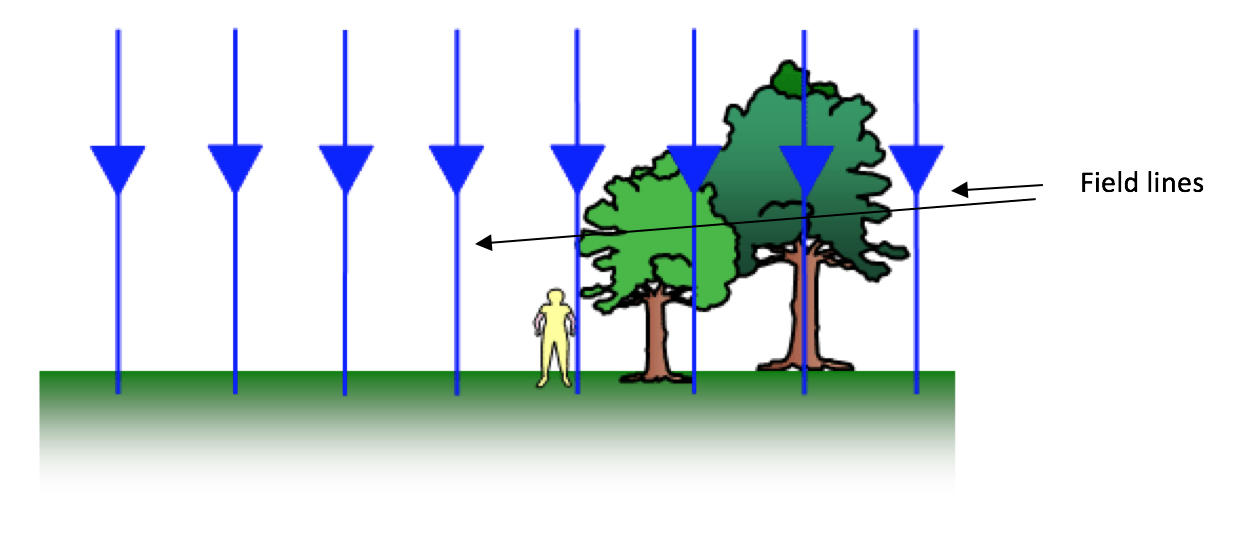
\includegraphics[width=\textwidth]{figs/chapt-2/figure-1.png}
	\end{center}
	\caption{Uniform Field}
\end{figure}

As you can see, the field lines are \textbf{parallel} and
\textbf{evenly-spaced.} This is always the case for a uniform field.

\spec{explain the distinction between gravitational field strength and force and explain the concept that a field has independent properties.}

There is a very important distinction to make between
\textbf{gravitational field strength} and \textbf{force} at this point:
The field strength at any point is the same for all bodies in the field
and is the force felt per kilogram, but the force is different and
depends on the size of the mass there.

This is best illustrated with an example: If a mass of 60kg is in the
Earth's gravitational field at the surface of the Earth, then we can
calculate the force acting on it, its weight, using equation (3):

\[W = mg = \SI{60}{\kg} \times \SI{9.8}{\N\per\kg} = \SI{590}{\N}\]

So the force felt by the 60kg mass is 590N but the field strength for
the mass \textbf{and for any other mass} is 9.8Nkg\textsuperscript{-1}.
So the field strength is fixed by your position in the field and the
size of the mass that is exerting the field, and nothing else. The force
depends on the mass in the field as well.

\end{document}
